\documentclass[10pt,handout,compress]{beamer}
%\documentclass[10pt]{beamer}
%% Class options include: notes, notesonly, handout, trans,
%%                        hidesubsections, shadesubsections,
%%                        inrow, blue, red, grey, brown
%
%% Theme for beamer presentation.
\usepackage{beamerthemesplit}
\usepackage{natbib}    %number and author-year style referencing

\usepackage{times,epsfig,makeidx,amsfonts,amsmath,dcolumn,enumerate,multirow,graphicx,amssymb,colortbl,bm,pifont,color}
\usepackage[]{graphicx}
\usepackage{scalerel,amsfonts,bm}
\usepackage{graphicx}
\usepackage{animate}
\usepackage{xcolor}
\usepackage{hyperref}
\hypersetup{colorlinks=true,linkcolor=blue,urlcolor=blue}

\usepackage{listings}
\usepackage{fontawesome}

\newcommand*{\Scale}[2][4]{\scalebox{#1}{$#2$}}%
\setbeamertemplate{footline}[frame number]
%% Other themes include: beamerthemebars, beamerthemelined,
%%                       beamerthemetree, beamerthemetreebars
%
\newcommand{\balpha}{\bm{\alpha}}
\newcommand{\bbeta}{\bm{\beta}}
\newcommand{\bgamma}{\bm{\gamma}}
\newcommand{\btheta}{\bm{\theta}}
\newcommand{\pr}{{\mathbb P}}
\newcommand{\bx}{{\bf x}}
\newcommand{\by}{{\bf y}}
\newcommand{\bz}{{\bf z}}
\DeclareMathAlphabet{\pazocal}{OMS}{zplm}{m}{n}
\newcommand{\La}{\mathcal{L}}
\newcommand{\Lb}{\pazocal{L}}
\renewcommand*{\bibfont}{\footnotesize}
%%------------------------------------------------------------------------------------------------------------------------------------------------------------------
%
\title[]{Net Survival Analysis: Parametric Models}

\author[]{ \textbf{Francisco Javier Rubio \\
\faTwitter \,\,\, @FJavierRubio1}}





%
\date{}
%
%
%
%
%%------------------------------------------------------------------------------------------------------------------------------------------------------------------
\begin{document}


\begin{frame}
  \titlepage
\end{frame}

%\begin{frame}{Overview}
%\tableofcontents
%\end{frame}

\begin{frame}
\frametitle{Lecture Aims}
\begin{itemize}
\item To introduce the relative survival framework.
\item To introduce a general hazard structure.
\item To present an application in cancer epidemiology.
\item To discuss a challenge in the relative survival framework.
\end{itemize}
\end{frame}

\begin{frame}
\frametitle{Cancer Epidemiology}
\setbeamercovered{invisible}
\begin{itemize}
\item We are exposed to many forces of mortality: ageing, illnesses, natural disasters, accidents, crime, COVID19, and etcetera. 
\pause
\item Cancer represents a strong force of mortality that affects large groups of individuals in all countries.
\pause 
\item Cancer patients, the population of interest in cancer epidemiology, are exposed to the additional force of mortality due to cancer. 
\pause
\item The aim is to quantify the survival of cancer patients in order to compare cancer management in different countries. \pause Thus, we need to comparable quantities.
\end{itemize}
\end{frame}

%
%\begin{frame}[c]
%\frametitle{The Bridge of Life: Painting commissioned by Karl Pearson}
%\begin{figure}
%\begin{center}
%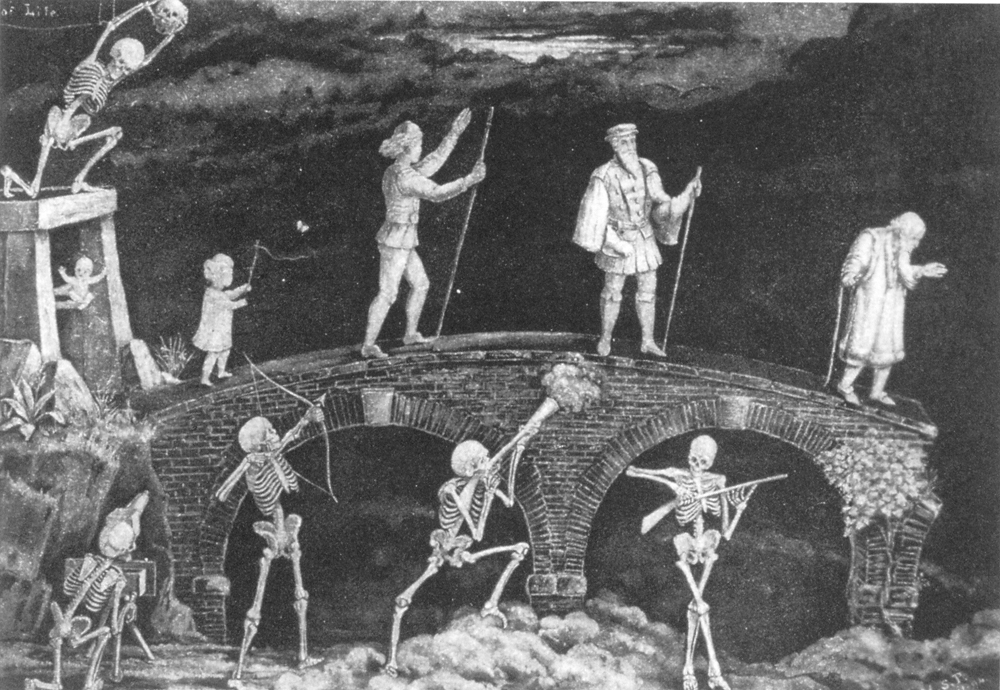
\includegraphics[scale=1]{Bridge}
%\end{center}
%\end{figure}
%\end{frame}

%
%\begin{frame}
%\frametitle{Human Mortality}
%\begin{figure}
%\begin{center}
%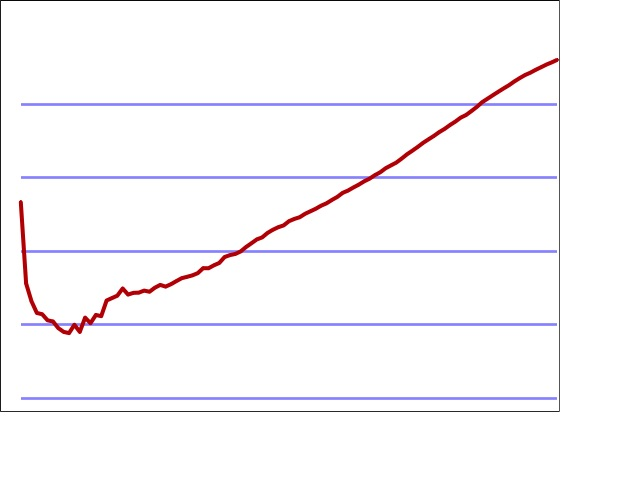
\includegraphics[scale=0.4]{LT}
%\end{center}
%\end{figure}
%\end{frame}

\begin{frame}
\frametitle{The typical data set}
\begin{itemize}
\item Sample of \textbf{times to event} (possibly right-censored) $(t_1,\ldots,t_n)$ from a group of individuals.
\pause
\item Vital status (or \textbf{censoring} indicators) $(\delta_1,\ldots,\delta_n)$. ($\delta_i=1$: death, $\delta_i=0$, right-censored/alive). \pause Censoring may be due to random drop-out, lost to follow-up, or administrative censoring.
\pause
\item In some cases, we may know some additional characteristics about the individuals, meaning we have access to \textbf{covariates} ${\bf x}_i = (x_{i1},\ldots,x_{i}p)^{\top}$, (age, sex, deprivation level, comorbidities, tumour stage, $\ldots$).
\end{itemize}
\end{frame}

\begin{frame}
\frametitle{Survival Analysis Frameworks}
\begin{itemize}
\item There are three approaches to analyse survival data:\pause
\begin{enumerate}
  \item The overall survival framework: all-cause mortality is analysed. \pause Not useful for comparison between populations as they are exposed to different causes of mortality. \pause
  \item The cause-specific framework: where the cause of death is known. \pause Death certificates are highly unreliable in all countries. \pause
  \item The relative survival framework: where we separate the \textcolor{blue}{hazard associated to other causes} and the \textcolor{red}{hazard associated to cancer}.
\end{enumerate}
\end{itemize}
\end{frame}



\begin{frame}
\setbeamercovered{invisible}
\frametitle{Relative survival framework}
\begin{itemize}
\item We would like to quantify the \textcolor{red}{mortality hazard due to the cancer} under study, and link this to the patients' characteristics. \pause

\item In the relative survival framework, we assume that the \textcolor{blue}{expected mortality hazard} (other causes than cancer) can be obtained from the general \href{https://www.ons.gov.uk/peoplepopulationandcommunity/birthsdeathsandmarriages/lifeexpectancies/datasets/nationallifetablesunitedkingdomreferencetables}{[population life tables]}.
\end{itemize}
\end{frame}



\begin{frame}
\frametitle{Excess mortality hazard regression models}
\setbeamercovered{invisible}
\begin{itemize}
\item More specifically, we can decompose the individual observed hazard, $h_o(\cdot;\cdot)$, as \pause
\begin{eqnarray}\label{HazardAddModel}
h_o(t;\bx) = \textcolor{blue}{h_P(A+t;\bz)} + \textcolor{red}{h_E(t;\bx)},
\end{eqnarray}
where $A=\text{age}$ (at diagnosis),  $\textcolor{blue}{h_P(A+t;\bz)}$ is the population hazard and it is obtained from the lifetables ($\bz \subset \bx$, age, sex, deprivation, $\ldots$), and $\textcolor{red}{h_E(t;\bx)}$ is the excess hazard. \pause

\item Assumptions:
\begin{itemize}
\item \textcolor{blue}{The general population hazard is supposed to correctly reflect the other-causes hazard in our population of interest.}%, assuming that the contribution in the general population hazard of the disease of interest is small compared to all others.
\item \textcolor{red}{The excess hazard is interpreted as the hazard due to the cancer under study.}
\end{itemize}
\end{itemize}
\end{frame}


\begin{frame}
\frametitle{Background Mortality}
\setbeamercovered{invisible}
\begin{itemize}
\item In order to calculate $\textcolor{blue}{h_P(A+t;\bz)} $, we need to get access to the life tables produced by the country where the patients live in. These are publicly available.
\pause
\item Depending on the country, these life tables are defined by different characteristics $\bz$. Typically: age, sex, and year.
\pause
\item In the UK, life tables are also available by Deprivation Level (I--V).
\pause
\item Example: Patient with characteristics $\bz_i = (\text{age} = 70, \text{sex} = \text{male}, \text{Deprivation} = \text{III}, \text{Year of Diagnosis} = 2010)$ and $t_i = 1 year$ \pause $\longrightarrow$ 2011 Life table  \pause $\longrightarrow$ Extract the corresponding mortality rate.
\end{itemize}
\end{frame}


\begin{frame}
\frametitle{Net survival}
\setbeamercovered{invisible}
\begin{itemize}
\item The main quantity of interest is the \textbf{net survival}, which is the survival function associated to the excess hazard. Thus,

$$S_N(t;\bx) =  \exp\left\{ - \int_0^{t} \textcolor{red}{h_E(s;\bx)} ds\right\}.$$


\pause
\item This quantity only depends on the EHM and it is a useful quantity for comparing the performance of cancer management between countries/period because it is not affected by differences in population mortality hazards.
\pause 
\item Policy-making for cancer management is often based on the population net survival
$$S_N(t) =  \dfrac{1}{n}\sum_{i=1}^nS_N(t;\bx_i).$$



\end{itemize}
\end{frame}


\begin{frame}
\begin{figure}
\begin{center}
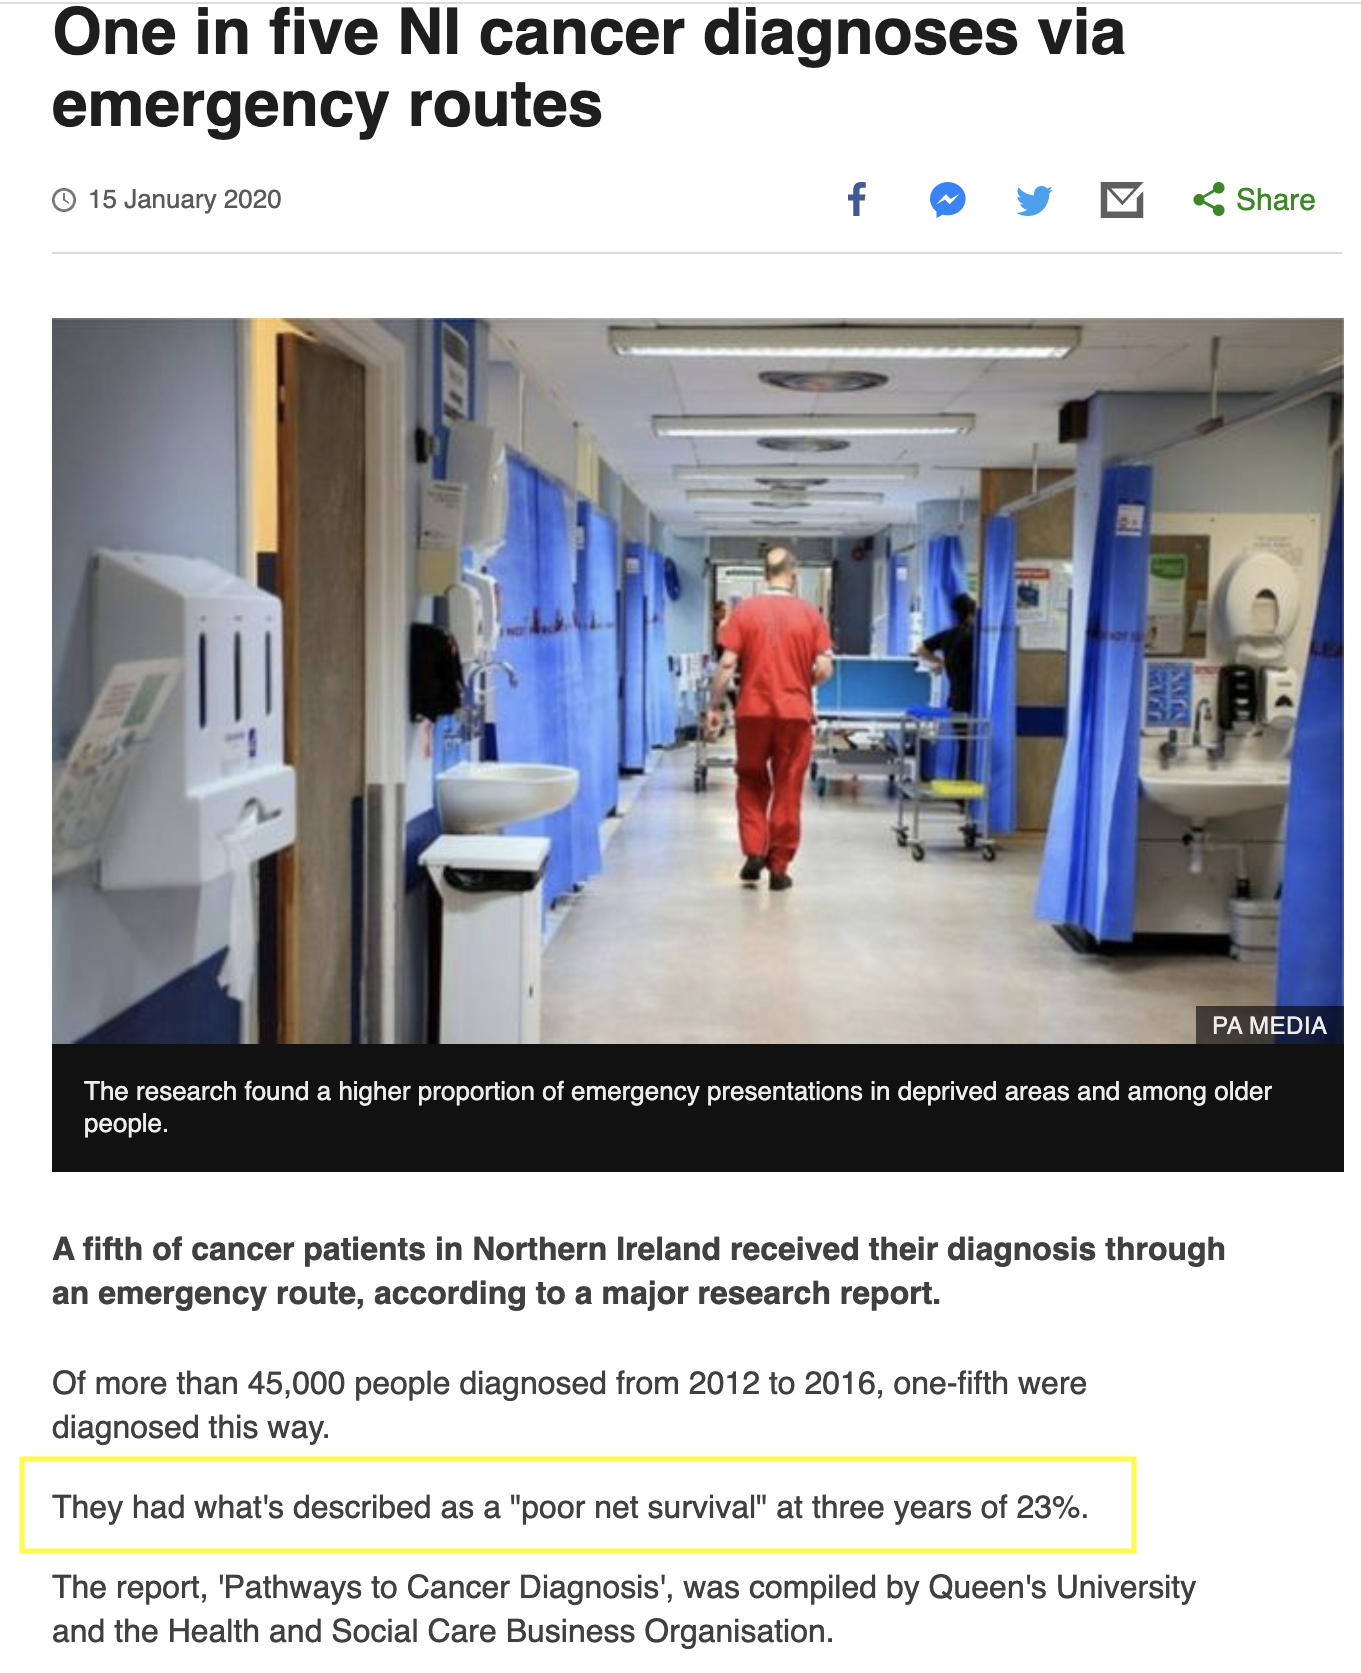
\includegraphics[scale=0.25]{bbc}
\end{center}
\end{figure}
\end{frame}


%\begin{frame}
%\frametitle{Estimators: Nonparametric}
%\setbeamercovered{invisible}
%\begin{itemize}
%\item The non-parametric estimator proposed by \citep{PS12} is perhaps the most popular in practice. \pause
%\item Adapted version of the Nelson-Aalen estimator.
%\pause
%\item It requires stratification of the data (\textit{e.g.}~by age group, which reduces the sample size), \pause and numerical integration.
%\end{itemize}
%\end{frame}


\begin{frame}
\frametitle{Which parametric excess hazard model?}
\setbeamercovered{invisible}
\begin{itemize}
\item Typically modelled as
$$h_E(t;\bx) = h_0(t)\exp\left(\bx^{\top}\bbeta\right).$$ 
%\pause
%
%\item  Semiparametric models using splines, nonparametric, and etcetera for modelling the baseline hazard. \pause They allow including time-dependent effects at the cost of one numerical integral per observation.

\pause

\item Fully Parametric models are of interest since they allow for prediction beyond the follow-up period, and they are typically more parsimonious models. 
\pause
\item The main criticisms are: (i) the PH assumption does not take into account time-varying effects, and (ii) the distributions used to model the baseline hazard can only cover specific shapes.
\end{itemize}
\end{frame}


\begin{frame}
\frametitle{The proposed model}
\setbeamercovered{invisible}
\begin{itemize}
\item Aims: (i) Consider more general alternatives to the PH structure, (ii) A parametric model which can cover the basic shapes of interest. \citep{R18}  \pause

\item (i) In order to avoid the proportional hazards model, we consider the general hazard (GH) structure \citep{C01}:

\begin{eqnarray}\label{GH}
h_{\text{E}}^{\text{G}}\left(t;\bx_i\right) &=& h_0\left(t \exp(\bx_i^{\top}\bbeta_1)\right)\exp(\bx_i^{\top}\bbeta_2), \pause \\
H_{\text{E}}^{\text{G}}\left(t;\bx_i\right) &\stackrel{Homework}{=}& H_0\left(t \exp(\bx_i^{\top}\bbeta_1)\right)\exp(\bx_i^{\top}\bbeta_2 - \bx_i^{\top}\bbeta_1).
\end{eqnarray}
\end{itemize}
\end{frame}

\begin{frame}
\begin{enumerate}[(i)]
\item If  $\bbeta_1=0$, then $\text{GH}=\text{PH}$.
\begin{eqnarray}\label{PH}
h_{\text{E}}^{\text{PH}}\left(t;\bx_i\right) &=& h_0(t)\exp\left(\bx_i^{\top}\bbeta\right).
\end{eqnarray}
\pause
\item if $\bbeta_2=0$, then $\text{GH}=\text{AH}$ (Accelerated hazards).
\begin{eqnarray}\label{AH}
h_{\text{E}}^{\text{AH}}\left(t;\bx_i\right) &=& h_0\left(t \exp(\bx_i^{\top}\bbeta)\right).
\end{eqnarray}
\pause
\item $\bbeta_1=\bbeta_2$, then $\text{GH}=\text{AFT}$ (Accelerated failure time).
\begin{eqnarray}\label{AFT}
h_{\text{E}}^{\text{AFT}}\left(t;\bx_i\right) &=& h_0\left(t \exp(\bx_i^{\top}\bbeta)\right)\exp(\bx_i^{\top}\bbeta).
\end{eqnarray}
\end{enumerate}
\end{frame}


\begin{frame}
\begin{itemize}
\item The GH structure also includes time-dependent effects through $\bbeta_1$.
\begin{center}
 \animategraphics[palindrome,autoplay,scale=0.5]{10}{h1-}{0}{59}
\end{center}
\end{itemize}
\end{frame}


\begin{frame}
\begin{itemize}
\item The GH structure also includes hazard-level effects through $\bbeta_2$.
\begin{center}
 \animategraphics[palindrome,autoplay,scale=0.5]{10}{h2-}{0}{59}
\end{center}
\end{itemize}
\end{frame}



\begin{frame}
\begin{itemize}
\item (ii) for the second aim, we will use the \href{https://rpubs.com/FJRubio/EWD}{[Exponentiated Weibull distribution]} \citep{M96}, which is defined as a simple transformation of the Weibull distribution $F(t \mid \kappa, \sigma)$:
$$G(t \mid \kappa, \sigma,\alpha) = F(t \mid \kappa, \sigma)^{\alpha},$$ \pause

\item This simple transformation adds a lot of flexibility since the corresponding hazard function can be: unimodal, increasing, decreasing, flat, bathtub. These shapes are often referred to as the ``basic shapes'' of the hazard function. \pause
\item By using the GH structure with EW baseline hazard, we cover both aims. $\checkmark$ \pause
\item There are some alternatives: generalised gamma, \href{https://rpubs.com/FJRubio/PGW}{[power generalised Weibull]}, and \href{https://rpubs.com/FJRubio/GWD}{[generalised Weibull]}.
%\pause
%\item We have checked the performance (bias, coverage, AIC for selecting the best structure) of this model using simulation as well as real data (UK).
\end{itemize}
\end{frame}

\begin{frame}
\frametitle{Maximum Likelihood Estimation}
\begin{itemize}
\item The likelihood function of the vector of parameters $\bm{\psi}$ is ${\mathcal L}_0(\bm{\psi};\text{Data})$
\begin{eqnarray*}
 &=& \prod_{i=1}^n h(t_i;\bx_i)^{\delta_i}S(t_i;\bx_i), \pause \\
  &=& \prod_{i=1}^n h(t_i;\bx_i)^{\delta_i}\exp\left\{-H(t_i;\bx_i)\right\}, \pause \\
&=& \prod_{i=1}^n \left\{ \textcolor{blue}{h_{\text{P}}(\text{age}_j+t_i;\bz_j)}+ \textcolor{red}{h_{\text{E}}(t_i;\bx_i)} \right\}^{\delta_i}\\
&\stackrel{Homework}{\times}& \exp\left\{- [\textcolor{blue}{H_{\text{P}}(\text{age}_j+t_i;\bz_j) -H_{\text{P}}(\text{age}_j;\bz_j)}]\right\} \exp\left\{- \textcolor{red}{H_{\text{E}}(t_i;\bx_i)}\right\}\\ \pause
&\propto& \prod_{i=1}^n \left\{ \textcolor{blue}{h_{\text{P}}(\text{age}_j+t_i;\bz_j)}+ \textcolor{red}{h_{\text{E}}(t_i;\bx_i)} \right\}^{\delta_i} \exp\left\{- \textcolor{red}{H_{\text{E}}(t_i;\bx_i)}\right\}.
\end{eqnarray*}
\end{itemize}
\end{frame}


\begin{frame}
\frametitle{Software and Examples}
\begin{itemize}
\item The GH model is implemented in the overall survival and relative survival frameworks in the R package \href{https://github.com/FJRubio67/GHSurv}{[GHSurv]}.

\item A manual on how to simulate times to event from the GH structure can be found at:

\url{https://rpubs.com/FJRubio/GHSim}

\item A simulated data example can be found at:

\url{https://rpubs.com/FJRubio/GHGH}

\item A manual on how to simulate times to event from a life table can be found at \href{https://github.com/FJRubio67/SimLT}{[SimLT]}.
\end{itemize}
\end{frame}

\begin{frame}
\frametitle{Real Data Application}
\begin{itemize}
\item We analysed a dataset obtained from population-based national cancer registry of lung cancer patients diagnosed in 2012 in the United-Kingdom.
\pause
\item We restricted our analysis to women with no missing data.
\pause
\item We observed $n = 14557$ patients with complete cases among which $n_o = 12138$ died before the 31st of December 2015.
\pause
\item The median follow-up among patients censored was $3.46$ years.
\end{itemize}
\end{frame}

\begin{frame}
\frametitle{Covariates}
\begin{itemize}
\item \textbf{Age at diagnosis}. The $25\%$, $50\%$ and $75\%$ quantiles of the patients' age at diagnosis was $64.9$, $72.6$, $80.2$ while the mean was $72.0$.
\item \textbf{Tumour stage (I--IV)}. $2434$ were Stage I, $1131$ were Stage II, $3421$ were Stage III, and $7751$ were Stage IV. 
\item \textbf{Income Score} (Income Domain from the 2010 England Indices of Multiple Deprivation). Continuous (0,1).
\item The presence of cardiovascular diseases (\textbf{Comorbidity}). $4318$ patients were classified with comorbidity indicator 1. 
\end{itemize}
\end{frame}



\begin{frame}
\frametitle{Model}
\begin{itemize}
\item We use the EW baseline hazard (3 parameters).
\pause
\item We fit 4 models for the excess hazard: PH, AFT, AH, GH.
\pause
\item Optimisation of the likelihood function is done using the R command {\tt optim}.
\pause
\item We will select a model using AIC.
\end{itemize}
\end{frame}


\begin{frame}
\begin{figure}
\begin{center}
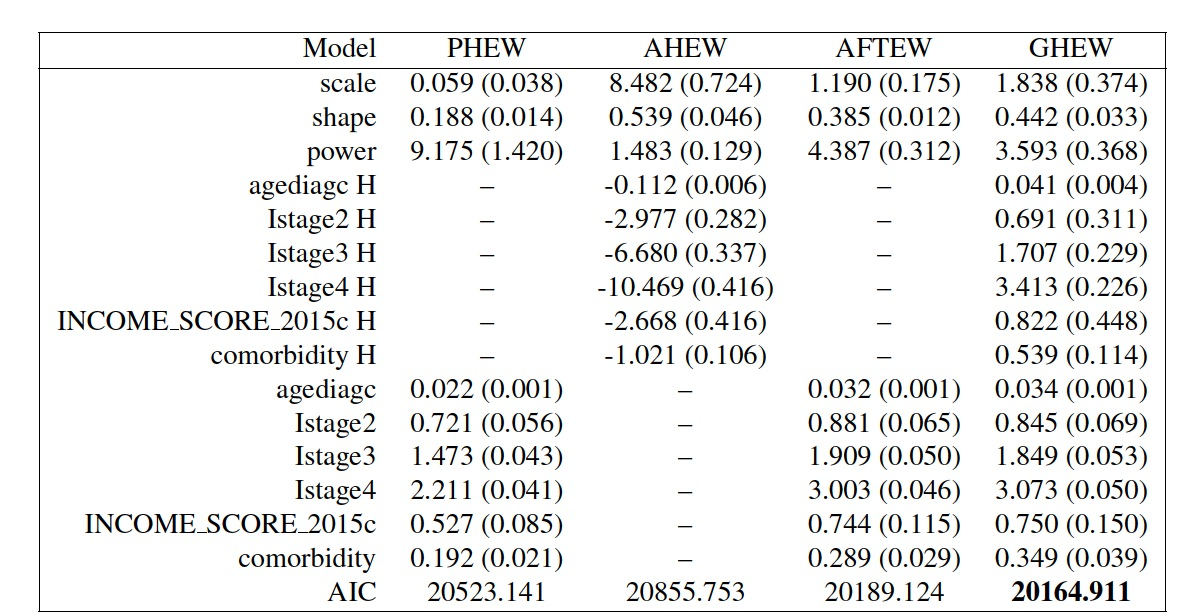
\includegraphics[scale=0.25]{table}
\end{center}
\end{figure}
\end{frame}

\begin{frame}
\frametitle{Net survival}
\begin{itemize}
\item We will now calculate the Net Survival at $t=1,2,3,3.9$ years after the diagnosis for two groups:
\begin{enumerate}
\item Total population by comorbidity $\{0,1\}$.
\item Age group 55-65 at Stage I by comorbidity $\{0,1\}$.
\end{enumerate} 
\pause
\item We will compare the estimates obtained with the selected parametric model with those obtained with a nonparametric estimator proposed by \cite{PS12}. This estimator is known as the Pohar-Perme estimator.
\end{itemize}
\end{frame}

\begin{frame}
\begin{figure}
\begin{center}
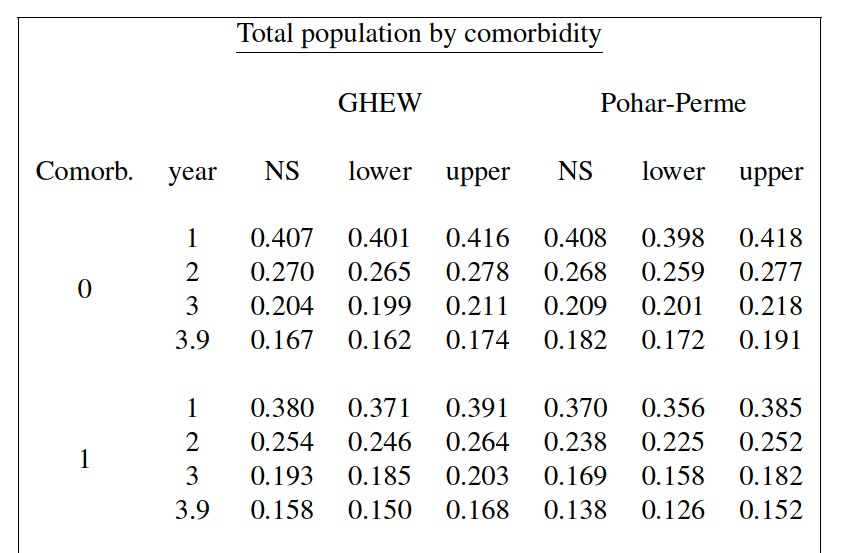
\includegraphics[scale=0.3]{NS1}
\end{center}
\end{figure}
\end{frame}

\begin{frame}
\begin{figure}
\begin{center}
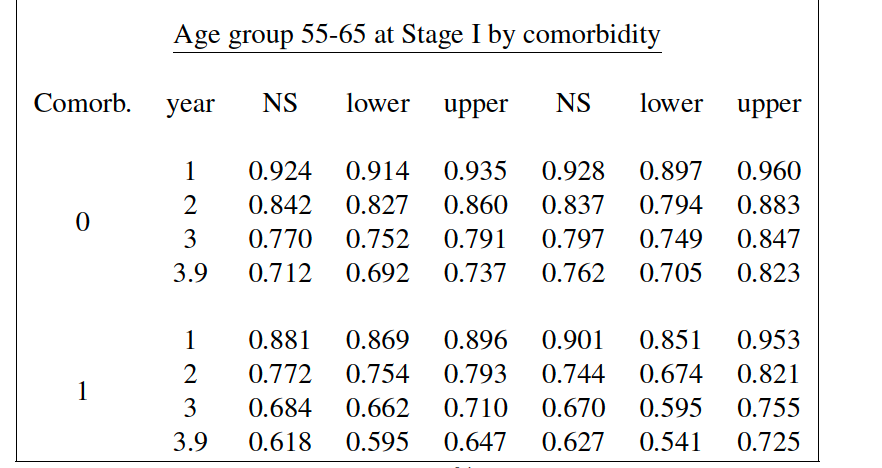
\includegraphics[scale=0.3]{NS2}
\end{center}
\end{figure}
\end{frame}

\begin{frame}
\frametitle{Discussion}
\begin{itemize}
\item We have studied the overall and relative survival frameworks. There are underlying assumptions in each of them. 
\pause
\item Survival parametric models are useful and interpretable tools for modelling time to event data. \pause It is important to understand the underlying assumptions of these models.
\pause
\item We have focused on the parametric framework, however, it is also possible to estimate survival functions using semi- and non- parametric approaches.
\pause
\item The relative survival framework is popular in policy making, thus it is important to have ``good models'' (try to reflect about what would make a good model).
\pause
\item Other challenges: Different types of censoring, informative censoring, competing risks, cure/remission models. Survival analysis is a vast area of active research (see \cite{eletti:2022}). 
\pause
\item In fact ...
\end{itemize}
\end{frame}


\begin{frame}
\frametitle{A challenge in the relative survival framework}
\begin{itemize}
\item We have assumed that
\begin{eqnarray*}
h_o(t;\bx) = \textcolor{blue}{h_P(A+t;\bz)} + \textcolor{red}{h_E(t;\bx)},
\end{eqnarray*}
\pause  the \textcolor{blue}{hazard associated to other causes} and the \textcolor{red}{hazard associated to cancer}.
\pause
\item In some countries, life tables are stratified by age, sex and year of diagnosis.
\pause
\item Then, in those countries, an extremely poor and an extremely rich patient with the same age, sex and year will be assigned the same $\textcolor{blue}{h_P(A+t;\bz)}$.
\end{itemize}
\end{frame}


\begin{frame}
\frametitle{A challenge in the relative survival framework}
\begin{itemize}
\item The same happens for a person with diabetes \emph{vs.}~a person without diabetes.
\pause
\item Thus, the population hazard is either overestimated or underestimated. 
\pause
\item A more detailed study of this challenge can be found in \cite{R19}.
\end{itemize}
\end{frame}

%
%
%\begin{frame}
%\frametitle{Insufficiently stratified life tables}
%\setbeamercovered{invisible}
%\begin{itemize}
%\item In many countries, life tables are only stratified by age, sex, and year. \pause
%\item This implies that patients sharing age, year of diagnosis, and sex, are assigned the same background mortality. \pause
%\begin{itemize}
%\item most-deprived and least-deprived patients,
%\item Smokers and non-Smokers,
%\item Diabetes, Cardiovascular diseases, ...
%\end{itemize}
%\pause
%\item The corresponding population hazard is either underestimated or overestimated.
%\end{itemize}
%\end{frame}
%
%\begin{frame}
%\frametitle{Single parameter correction}
%\begin{itemize}
%\item \cite{CR91} proposed a single-parameter correction
%\begin{eqnarray*}
%h_o(t;\bx \mid \textcolor{gray}{\bm{\eta}}) &=& \textcolor{gray}{\bm{\eta}}\textcolor{blue}{h_P(A+t;\bz)} + \textcolor{red}{h_E(t;\bx)},
%\end{eqnarray*}
%where $\textcolor{gray}{\bm{\eta}}>0$ is an unknown parameter.\pause
%\item They adopt a proportional excess hazard model.
%\pause
%\item It assumes that the correction is constant for all the patients, which is rather unrealistic in population studies.
%\end{itemize}
%\end{frame}
%
%\begin{frame}
%\frametitle{Including covariates in the SPC}
%\begin{itemize}
%\item In order to alleviate this assumption, \cite{T19} proposed modelling $\eta$ in terms of available covariates.
%\pause
%\item This allows for a different indivual correction. \pause However, it imposes a specific model for the inclusion of these variable $\eta_i = \exp(x_i^{\top}\theta)$.
%\pause
%\item Perhaps more importantly, not all relevant variables may be available.
%\end{itemize}
%\end{frame}
%
%\begin{frame}
%\frametitle{Correlated Frailty Model}
%\begin{itemize}
%\item \cite{Z97} proposed a correlated frailty model, by using frailties on both the population hazard and the excess hazard:
%\begin{eqnarray}\label{CFM}
%h_o^{Z}(t;\bx\vert \gamma_1,\gamma_2) &=& h_P(A+t;y+t,\bz)\textcolor{purple}{\gamma_1} + h_E(t;\bx)\textcolor{purple}{\gamma_2},
%\end{eqnarray}
%where $(\textcolor{purple}{\gamma_1,\gamma_2})\sim G_2$, and $G_2$ is a bivariate distribution with support on the positive quadrant.
%\pause
%\item  \cite{Z97} found that the maximum likelihood estimators of the parameters of model \eqref{CFM} do not exist, suggestive of identifiability issues of this model.
%\pause
%\item  \cite{Z97} proposed truncating the parameter space to a compact set. This did not solve the identifiability issues.
%\end{itemize}
%
%\end{frame}
%
%
%
%\begin{frame}
%\frametitle{The proposed correction}
%\begin{itemize}
%\item \cite{R19} propose a solution to this problem is to add a random correction (frailty): \pause
%\begin{eqnarray*}
%h_o(t;\bx \mid \textcolor{brown}{\bm{\eta}}) &=& \textcolor{brown}{\bm{\eta}}\textcolor{blue}{h_P(A+t;\bz)} + \textcolor{red}{h_E(t;\bx)},\\
%\textcolor{brown}{\bm{\eta}} &\sim& G.
%\end{eqnarray*}
%%where $\mu$ is the unknown mean and $b$ is the unknown scale.
%\item \textcolor{brown}{Individual-level correction.}
%\item \textcolor{brown}{The correction is non-specific.}
%\item \textcolor{brown}{The correction only applies to the population hazard.}
%\end{itemize}
%\end{frame}
%
%
%\begin{frame}
%\frametitle{The marginal survival function}
%Integrating out the frailty $\eta$ with respect to the distribution $G$, the individual marginal survival function can be written as
%\begin{eqnarray}
%\tilde{S}_o(t;\bx) = \exp\{-\textcolor{red}{H_E(t;\bx)}\}\Lb_G\{\textcolor{blue}{H_P(A+t;y+t;\bz) - H_P(A;y;\bz)}\},
%\end{eqnarray}
%where $\Lb_G\{s\} = \int_0^{\infty} e^{-s  r}dG(r)$ denotes the Laplace transform of $G$ evaluated at time $s$.
%\end{frame}
%
%\begin{frame}
%\begin{itemize}
%\item Good news: We know distributions with a closed-form Laplace transform.
%\pause
%\item Bad news: we pretty much only know two families -- Gamma (2-parameters), Power Variance Function (3-parameters).
%
%\pause
%\item
%\begin{eqnarray*}
%\textcolor{brown}{\bm{\eta}} &\sim& Gamma(\mu,b),
%\end{eqnarray*}
%where $\mu$ is the unknown mean and $b$ is the unknown scale
%\end{itemize}
%
%\end{frame}
%
%
%
%\begin{frame}
%
%\begin{itemize}
%\item The hazard has a tractable expression:
%\begin{eqnarray*}
%\tilde{h}_o(t;\bx) =  \dfrac{\textcolor{brown}{\mu} \, \textcolor{blue}{h_P(A+t;y+t;\bz)}}{\textcolor{brown}{1+b \left[H_P(A+t;y+t;\bz)-H_P(A;y;\bz)\right]}} + \textcolor{red}{h_E(t;\bx)}.
%\end{eqnarray*}
%\item The marginal individual survival function is given by
%\begin{eqnarray}\label{OverSurv1}
%\tilde{S}_o(t;\bx) &=& \dfrac{\exp\left\{- \textcolor{red}{H_E(t;\bx)}\right\} }{\left\{1+b \left[\textcolor{blue}{H_P(A+t;y+t;\bz)-H_P(A;y;\bz)}\right]\right\}^{\frac{\mu}{b}}}.
%\end{eqnarray}
%\end{itemize}
%\end{frame}
%
%
%
%\begin{frame}
%\frametitle{Likelihood functions}
%\begin{itemize}
%\item Classical model:
%
%\begin{eqnarray*}
%	{\mathcal L}(\bm{\psi};\text{Data}) &=& \prod_{i=1}^n {h}_o(t_i;\bx_i)^{\delta_i}{S}_o(t_i;\bx_i)\\
%	&\propto& \prod_{i=1}^n \left\{ h_P(A_i+t_i; y_i + t_i, \bz_i) + h_E(t_i;\bx_i) \right\}^{\delta_i} \\
%	&\times&\exp\left\{- H_E(t_i;\bx_i)\right\},
%\end{eqnarray*}
%\end{itemize}
%\end{frame}
%
%
%\begin{frame}
%\frametitle{Likelihood functions}
%\begin{itemize}
%\item Single parameter correction:
%\begin{eqnarray*}
%{\mathcal L}_C(\bm{\psi}_C;\text{Data}) &=& \prod_{i=1}^n \left\{\eta h_P(A_i+t_i;y_i+t_i;\bz_i) + h_E(t_i;\bx_i) \right\}^{\delta_i} \\
%&\times& \exp\left\{- H_E(t_i;\bx_i)\right\} \\
%&\times& \exp\{-[H_P(A_i+t_i;y_i+t_i;\bz_i)-H_P(A_i;y_i;\bz_i)]\}^{\eta},
%\end{eqnarray*}
%where $\bm{\psi}_C = (\eta, \bm{\psi})$.
%\end{itemize}
%\end{frame}
%
%
%\begin{frame}
%\frametitle{Likelihood functions}
%\begin{itemize}
%\item Frailty correction model ${\mathcal L}_F(\bm{\psi}_F;\text{Data})=$
%\begin{eqnarray*}\label{LogLikM3}
%&& \prod_{i=1}^n \left\{ \dfrac{\mu \, h_P(A_i+t_i;y_i+t_i;\bz_i)}{1 + b \left[H_P(A_i+t_i;y_i+t_i;\bz_i)-H_P(A_i;y_i;\bz_i)\right]} + h_E(t_i;\bx_i) \right\}^{\delta_i} \\ &\times&\dfrac{\exp\left\{- H_E(t_i;\bx_i)\right\} }{\left\{1 + b \left[H_P(A_i+t_i;y_i+t_i;\bz_i)-H_P(A_i;y_i;\bz_i)\right]\right\}^{\frac{\mu}{b}}},
%\end{eqnarray*}
%where $\bm{\psi}_F = (\mu,b,\bm{\psi})$.\pause
%\item We can estimate the parameters using likelihood methods.
%\end{itemize}
%\end{frame}
%
%\begin{frame}
%\frametitle{There ain't no such thing as a free lunch}
%\begin{itemize}
%\item The information about the frailty parameters comes from the differences in population cumulative hazards. Not an easy task to calculate them.
%\pause
%\item We model the excess hazard parametrically as in the first part, and obtain an identifiable model.
%\pause
%\item An extensive simulation study suggests that we need at least $5,000$ observations (unfortunately, not an onerous condition in cancer epidemiology), and less than $50\%$ censoring rate.
%\end{itemize}
%\end{frame}
%
%
%\begin{frame}
%\frametitle{Why bother about corrections?}
%\begin{itemize}
%\item Extra effort is justified by the fact that mismatched life tables may produce biased net survival.
%\pause
%\item We have explored cases where this is the case, using simulations, as well as cases where a correction is not necessary. \pauses These cases were identified using model selection.
%\end{itemize}
%\end{frame}
%
%
%
%
%\begin{frame}
%\frametitle{Real Data Example}
%\begin{itemize}
%\item We analysed a dataset obtained from population-based national cancer registry of Non-Small Cell Lung Cancer (NSCLC) patients diagnosed in 2012 in England.
%\pause
%\item We restricted our analysis to men with no missing data. We observed $n=15688$ patients with complete cases among which $n_o=13603$ died before the 31st of December 2015.
%\pause
%\item We used life tables based on age, sex, year, and deprivation level.
%\end{itemize}
%\end{frame}
%
%\begin{frame}
%
%\begin{table}[]
%{\scriptsize	
%	\centering
%	\begin{tabular}{|rlll|}
%		\hline
%		& M1 & M2 & M3  \\
%		\hline
%  $b$ & -- & -- & 9.83 (3.03)  \\
%  $\gamma \mid \mu$ & -- & 2.7 (0.21) & 6.54 (0.91) \\
%  $\theta$ & 0.05 (0.01) & 0.03 (0.01) & 0.03 (0.01)  \\
%  $\kappa$ & 0.38 (0.01) & 0.35 (0.01) & 0.34 (0.01)  \\
%  $\alpha$ & 4.64 (0.34) & 5.64 (0.48) & 5.92 (0.58)  \\
%  Age-t & 0.29 (0.04) & 0.29 (0.04) & 0.16 (0.05)  \\
%  Dep-t & 0.11 (0.04) & 0.12 (0.04) & 0.09 (0.04)  \\
%  Stage 1-t & -2.66 (0.25) & -2.17 (0.32) & -5.4 (1.4)  \\
%  Stage 2-t & -2.2 (0.2) & -2 (0.22) & -2.69 (0.35)  \\
%  Stage 3-t & -1.66 (0.11) & -1.57 (0.11) & -1.75 (0.13)  \\
%  CV-t & \textcolor{orange}{0.31} (0.11) & 0.31 (0.11) & \textcolor{orange}{0.42} (0.11) \\
%  COPD-t & \textcolor{orange}{0.13} (0.11) & 0.08 (0.12) & \textcolor{orange}{0.37} (0.14)  \\
%  Age & 0.27 (0.01) & 0.23 (0.02) & 0.16 (0.02)  \\
%  Dep & 0.06 (0.01) & 0.06 (0.01) & 0.04 (0.01)  \\
%  Stage 1 & -2.84 (0.06) & -3.13 (0.1) & -3.53 (0.36)  \\
%  Stage 2 & -2.16 (0.06) & -2.32 (0.07) & -2.65 (0.1)  \\
%  Stage 3 & -1.23 (0.03) & -1.27 (0.04) & -1.36 (0.04)  \\
%  CV & \textcolor{orange}{0.24} (0.04) & 0.26 (0.04) & \textcolor{orange}{0.3} (0.04)  \\
%  COPD & \textcolor{orange}{0.19} (0.04) & 0.17 (0.04) & \textcolor{orange}{0.25} (0.05)  \\
%  AIC & 20304.69 & 20241.27 & {\bf 20213.41} \\
%  \hline
%	\end{tabular}
%%\caption{\small Regression parameter estimates (standard errors) using models M1--M3, with their corresponding AIC on the men lung cancer dataset. Note: The time- dependent effects are indicated with ‘-t’. For model M2, $\gamma$ is estimated, while $\mu$ is estimated for model M3. Age=Age at diagnosis (centred at 70, and divided by 10), Dep=Income Deprivation Score (centred at 0.1, and divided by 10), CV=CardioVascular comorbidity, COPD=Chronic Obstructive Pulmonary Disease, AIC=Akaike Information Criteria (best model indicated in bold font).}
%%\label{table:betahat}
%}
%\end{table}
%\end{frame}
%
%\begin{frame}
%\begin{figure}[]
%	\begin{center}
%		\begin{tabular}{c}
%			\includegraphics[scale=0.35,angle=-90]{gph_stage2_stage4_withDep_RevisedPaper.eps}
%		\end{tabular}
%	\end{center}
%	\caption{\scriptsize Men, 70 years old at diagnosis, Least deprived, without Cardiovascular comorbidity nor COPD, and Stage IV (upper panels) or Stage II (lower panels). M1=solid grey lines, M2=dot-dashed black lines, M3=long-dashed black lines}
%	\label{fig:EMH_NS}
%\end{figure}
%
%\end{frame}
%
%\begin{frame}
%\frametitle{Quick interpretation}
%\begin{itemize}
%\item We observe that the frailty distribution, used for correcting the population mortality in M3, cumulates $23\%$ of the probability mass below $1$, and $77\%$  above $1$.
%\pause
%\item These values are in fact related to the proportion of smokers (roughly $80\%$, which would, in principle, require a correction higher than 1) for England lung cancer patients, based on hospital data.
%\pause
%\item The impact of the presence of a comorbidity is
%higher in M3 compared to M1 and M2. \pause Thus, correcting the population life table for unobserved predicting variables of background mortality seems to be quite relevant in this example.
%\end{itemize}
%
%\end{frame}
%
%
%\begin{frame}
%\frametitle{The Ugly: Specific Life Tables}
%\begin{figure}
%\begin{center}
%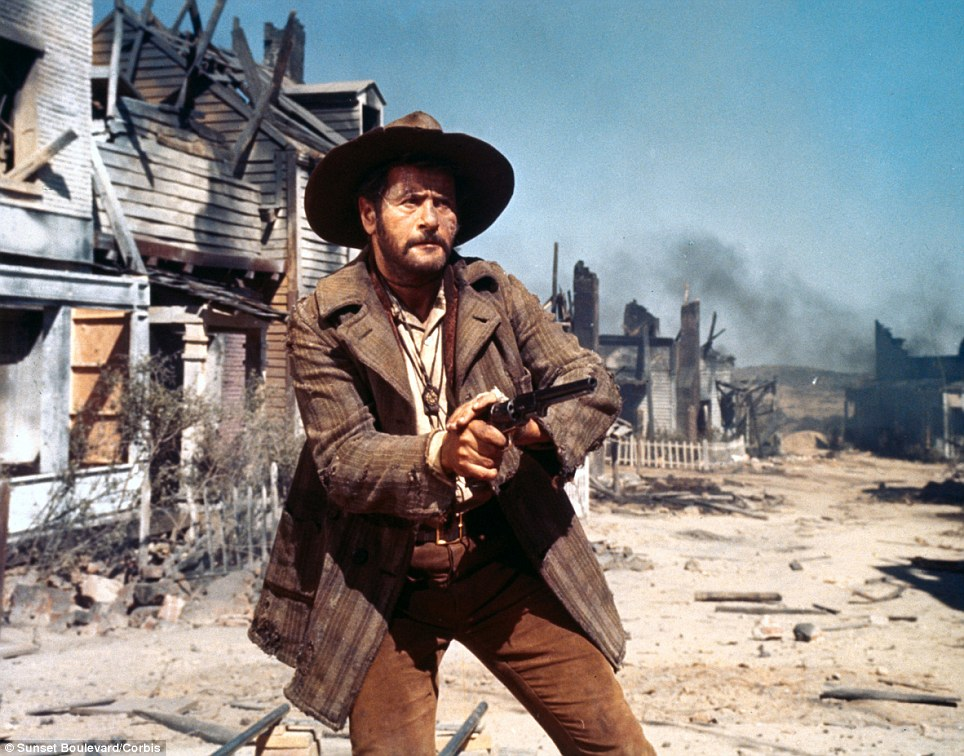
\includegraphics[scale=0.25]{ugly}
%\end{center}
%\end{figure}
%\end{frame}
%
%
%
%\begin{frame}
%\setbeamercovered{invisible}
%\begin{itemize}
%\item The Good. There is room for improvement in modelling.
%\pause
%\item The Bad. There is a challenging mismatch that may affect conclusions.
%\pause
%\item What should we do: to correct the population hazard or to try to get better life tables? \pause
%\item By comorbidity, by drug use (smokers vs. non-smokers), ... \pause
%\item How far can we go in terms of stratifying the life tables? Additional stratification reduces the sample size at each subgroup. \pause Shall we stop at some point? If so, at what point?
%\pause
%\item Elephant in the room: Is net survival the best way of comparing cancer management between countries? \pause Is survival in general the best tool?
%
%\end{itemize}
%\end{frame}


%\begin{frame}<beamer:0>
\bibliographystyle{plainnat}
\bibliography{references}
%\end{frame}
\end{document}
%
%





